\documentclass[12pt,a4paper]{article}
\usepackage{multirow}
\usepackage{xeCJK}
\usepackage{amssymb}
\usepackage{amsmath}
\usepackage{mathtools}
\usepackage{geometry}
\usepackage{subfig}
\usepackage{fancyhdr}
\usepackage[export]{adjustbox}
\usepackage{graphicx}
\geometry{left=2.5cm,right=1.5cm,top=2cm,bottom=2cm}

\title{Self Driving Car \\HW2 \\ Report}
\date{March 20, 2019}
\author{呂紹篁, 0751904}
\setCJKmainfont{AR PL UKai CN}
\begin{document}
\thispagestyle{plain}
\cfoot{}
\maketitle
\paragraph{2}
Define random variable $\{X_t: \text{the weather of Day t}\}$ where the value $x_t=\begin{cases} 1: sunny \\ 2: cloudy \\ 3: rainy \end{cases}$ .
Given \textbf{transition matrix} $M = \\
\begin{bmatrix}
P(x_\text{t+1}=1|x_t=1) & P(x_\text{t+1}=1|x_t=2) & P(x_\text{t+1}=1|x_t=3) \\
P(x_\text{t+1}=2|x_t=1) & P(x_\text{t+1}=2|x_t=2) & P(x_\text{t+1}=2|x_t=3) \\
P(x_\text{t+1}=3|x_t=1) & P(x_\text{t+1}=3|x_t=2) & P(x_\text{t+1}=3|x_t=3) 
\end{bmatrix} =
			     \begin{bmatrix}
			      0.8 & 0.4 & 0.2 \\
                              0.2 & 0.4 & 0.6 \\
                              0   & 0.2 & 0.2
                             \end{bmatrix}$ \\
And using the notation $\overrightarrow{v_t}$ to represent the probability of weather at Day t.
\begin{itemize}

\item{(a)} 
%Given Day1 is sunny, using the notation $\overrightarrow{v_1} = {\begin{bmatrix} 1 & 0 & 0 \end{bmatrix}}^T$ to represent the prabability of weather of Day1, and DayN for $\overrightarrow{v_n}$. Then, intuitively, $\overrightarrow{v_n} = M^n*\overrightarrow{v_1}$, then we have 
%\begin{eqnarray} 
%  \left\{
%    \begin{aligned}
%      \overrightarrow{v_2}={\begin{bmatrix} 0.800 & 0.200 & 0.000 \end{bmatrix}}^T \\
%      \overrightarrow{v_3}={\begin{bmatrix} 0.720 & 0.240 & 0.040 \end{bmatrix}}^T \\
%      \overrightarrow{v_4}={\begin{bmatrix} 0.680 & 0.264 & 0.056 \end{bmatrix}}^T \\
%    \end{aligned}
%  \right.
%\end{eqnarray}
%Thus, \\ $P\{Day2=\textbf{cloudy}\} = 0.2$, \\ $P\{Day3=\textbf{cloudy}\} = 0.24$ and \\ $P\{Day4=\textbf{rainy}\} = 0.056$

The probability of the sequence \textit{\{Day2=cloudy, Day3=cloudy, Day4=rainy\}} is \\
$P(x_2=2|x_1=1)P(x_3=2|x_2=2)P(x_4=3|x_3=2)=0.2*0.4*0.2=\textbf{0.016}$
\item{(b)}
The screenshot of the simulator and an example output is shown in Fig~\ref{fig:sim}.
\begin{figure}[hbt]
  \centering
  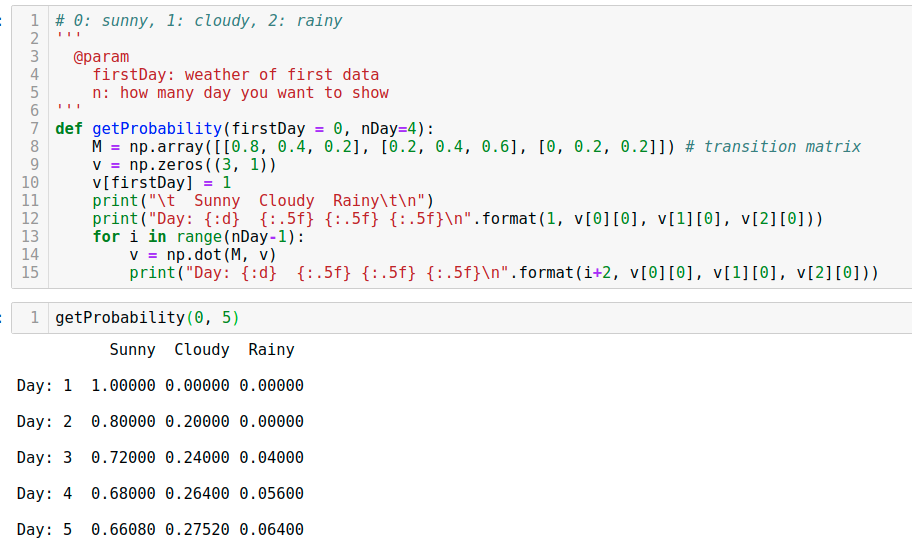
\includegraphics[scale=0.4]{simulator.png}
  \caption{Code of simulator and a sample result}
  \label{fig:sim}
\end{figure}
\item{(c)}
Using the simulator above with large number of day, the result 
$\overrightarrow{v_\text{steady}} = \lim\limits_{n \to \infty}\overrightarrow{v_n} = {\begin{bmatrix} 0.643 & 0.286 & 0.071 \end{bmatrix}}^T$
\item{(d)}
The result in (c) can be simpliy computed using eigenvalue decomposition, \\
$ 
  M = T\Lambda{T}^-1  \\ 
   = \begin{bmatrix}
     -0.909 & 0.813 & 0.233 \\
     -0.404 & -0.476 & -0.794 \\
     -0.101   & -0.337 & 0.562
     \end{bmatrix} * 
  \begin{bmatrix} 
    1 & 0 & 0 \\
    0 & 0.483 & 0 \\
    0 & 0 & -0.083
  \end{bmatrix} *
  {\begin{bmatrix}
     -0.909 & 0.813 & 0.233 \\
     -0.404 & -0.476 & -0.794 \\
     -0.101   & -0.337 & 0.562
     \end{bmatrix}}^{-1} \\
  M^n = T{\Lambda}^n{T}^{-1} \\
  = \begin{bmatrix}
     -0.909 & 0.813 & 0.233 \\
     -0.404 & -0.476 & -0.794 \\
     -0.101   & -0.337 & 0.562
     \end{bmatrix} *
  {\begin{bmatrix} 
    1 & 0 & 0 \\
    0 & 0.483 & 0 \\
    0 & 0 & -0.083
  \end{bmatrix}}^n *
  {\begin{bmatrix}
     -0.909 & 0.813 & 0.233 \\
     -0.404 & -0.476 & -0.794 \\
     -0.101   & -0.337 & 0.562
     \end{bmatrix}}^{-1}
$
Since two minor eigenvalues are smaller than 1, with large n, $\Lambda^n$ converges to 
$\begin{bmatrix}
1 & 0 & 0 \\
0 & 0 & 0 \\
0 & 0 & 0 \end{bmatrix}$ and thus M converges to \\
$
  \begin{bmatrix}
     -0.909 & 0.813 & 0.233 \\
     -0.404 & -0.476 & -0.794 \\
     -0.101   & -0.337 & 0.562
  \end{bmatrix} *
  {\begin{bmatrix} 
    1 & 0 & 0 \\
    0 & 0 & 0 \\
    0 & 0 & 0
  \end{bmatrix}}^n *
  {\begin{bmatrix}
     -0.909 & 0.813 & 0.233 \\
     -0.404 & -0.476 & -0.794 \\
     -0.101   & -0.337 & 0.562
   \end{bmatrix}}^{-1} \\
  = 
  \begin{bmatrix}
     0.643 & 0.643 & 0.643 \\
     0.286 & 0.286 & 0.286 \\
     0.071   & 0.071 & 0.071 
  \end{bmatrix}
$ \\
With arbitrary $\overrightarrow{v_1} \in \{ {\begin{bmatrix} 1 & 0 & 0 \end{bmatrix}}^T,
{\begin{bmatrix} 0 & 1 & 0 \end{bmatrix}}^T,
{\begin{bmatrix} 0 & 0 & 1 \end{bmatrix}}^T\} 
$ all converges to $\overrightarrow{v_\text{steady}}$ mentioned in (c).
\item{(e)}
$H = \displaystyle\sum_{x}^{} P(x)\log_2\frac{1}{P(x)} = 
\frac{9}{14}\log_2\frac{14}{9}+\frac{4}{14}\log_2\frac{14}{4}+\frac{1}{14}\log_214=\textbf{1.198}$
\item{(f)}
Define random varaibles \textit{x: today's weather} and \textit{y: tomorrow's weather}. By \textbf{Bayes's rule}, \\
$P(y|x) = \frac{P(x|y)P(y)}{P(x)} = \frac{P(x|y)P(y)}{\displaystyle\sum_{y'} P(x|y=y')P(y=y')}$ 
where y'= $\begin{cases} 1: sunny \\ 2: cloudy \\ 3: rainy \end{cases}$ \\
$P(x|y)$ can be obtained from the transition table, and for $P(y=y')$, we can get the value from (c).
After computation, 9 values with different x and y are shown in Table~\ref{tab:f}.
\item{(g)}
\textbf{Yes}, it will violate the Markov property since two adjacent days are not totally independent after the consideration of seasons.
\end{itemize}

\begin{table}[h]
\centering
\begin{tabular}{ll|lll}
\multicolumn{2}{l}{\multirow{2}{*}{}}         & \multicolumn{3}{l}{Today's weather} \\
\multicolumn{2}{l}{}                          & sunny      & cloudy     & rainy     \\
\hline
\multirow{3}{*}{Yesterday's weather} & sunny  & $\frac{72}{90}$      & $\frac{18}{36}$      & \small 0      \\
                                     & cloudy & $\frac{16}{90}$      & $\frac{16}{36}$      & $\frac{8}{10}$      \\
                                     & rainy  & $\frac{2}{90}$       & $\frac{2}{36}$       & $\frac{2}{10}$

\end{tabular}
\caption{Result of (f)}
\label{tab:f}
\end{table}

\paragraph{3}
Sensor model S = $\begin{bmatrix} 
P(z_t=1|x_t=1) & P(z_t=1|x_t=2) & P(z_t=1|x_t=3) \\
P(z_t=2|x_t=1) & P(z_t=2|x_t=2) & P(z_t=2|x_t=2) \\
P(z_t=3|x_t=1) & P(z_t=3|x_t=2) & P(z_t=3|x_t=3) \\
\end{bmatrix} \\
= \begin{bmatrix}
0.6 & 0.3 & 0 \\ 0.4 & 0.7 & 0 \\ 0 & 0 & 1
\end{bmatrix}$ \\
Define random variables \textit{$x_t$: weather at Day t} and \textit{$z_t$: sensor measurement at Day t} both values in set $\{1, 2, 3\}$. Weather belief $Bel(x_t)=P(x_t|z_1, z_2, ..., z_\text{t-1})$ tell our 'belief' that the weather at Day t given prior measurements.
\begin{itemize}
\item{(a)}
From the measurement table and the data, Day 4 must be rainny obviously., that is, $Bel(x_4=3)=1$. With Markov assumption, we can compute the belief of Day 5 from the fact that Day 4 is rainy directly. By \textbf{Bayes filter}, \\

$Bel(x_5=1)=\eta P(z_5=1|x_5=1)\displaystyle\sum_{x'}^{} P(x_5=1|x_4=x')Bel(x_4=x') \\ 
\qquad = \eta P(z_5=1|x_5=1)P(x_5=1|x_4=3)Bel(x_4=3) \\
\qquad = \eta 0.6*0.2 \\ = 0.12\eta$ 

$Bel(x_5=2)=\eta P(z_5=1|x_5=2)\displaystyle\sum_{x'}^{} P(x_5=2|x_4=x')Bel(x_4=x') \\ 
\qquad = \eta P(z_5=1|x_5=2)P(x_5=2|x_4=3)Bel(x_4=3) \\
\qquad = \eta 0.3*0.6 \\ = 0.18\eta$ 

$Bel(x_5=3)=0\because P(z_5=1|x_5=3)=0$

After normalization, we have $Bel(x_5=1)=0.4$ and $Bel(x_5=2)=0.6$ \\
So, the probability that Day 5 is indeed sunny is \textbf{0.4}.

\item{(b)} 
\subitem{Case 1} \\
Initial point: $ Bel(x_1=1)=1 \because \text{Day 1 already known}$ \\ \\
$ Bel(x_2=1)=\eta P(z_3=1|x_2=1)P(x_2=1|x_1=1)Bel(x_1=1)=\eta 0.6*0.8=0.48\eta$ \\ 
$ Bel(x_2=2)=\eta P(z_3=1|x_2=2)P(x_2=2|x_1=1)Bel(x_1=1)=\eta 0.3*0.2=0.06\eta$ \\
$ Bel(x_2=3)=\eta P(z_3=1|x_2=3)P(x_2=3|x_1=1)Bel(x_1=1)=0$ \\
After normalizaton, $ Bel(x_2=1)=\textbf{0.889}$ and $ Bel(x_2=2)= 0.111$ \\ \\

$ \scriptstyle Bel(x_3=1)=\eta P(z_3=1|x_3=1)[P(x_3=1|x_2=1)Bel(x_2=1)+P(x_3=1|x_2=2)Bel(x_2=2)]=0.453\eta$ \\
$ \scriptstyle Bel(x_3=2)=\eta P(z_3=1|x_3=2)[P(x_3=2|x_2=1)Bel(x_2=1)+P(x_3=2|x_2=2)Bel(x_2=2)]=0.067\eta$ \\
$ \scriptstyle Bel(x_3=3)=\eta \underline{P(z_3=1|x_3=3)}[P(x_3=3|x_2=1)Bel(x_2=1)+P(x_3=3|x_2=2)Bel(x_2=2)]=0$ \\
After normalizaton, $ Bel(x_3=1)=\textbf{0.872}$ and $ Bel(x_3=2)=0.128$ \\ \\
For Day 4, since the measurement is rainy and by the measurement model, \\ $ Bel(x_4=3)=\textbf{1}$ without doubt.

\subitem{Case 2} \\

With the knowledge of future data, \\
$\scriptstyle P(x_2=1|z_\text{2:4})= \eta P(z_2=1|x_2=1, z_\text{3:4})P(x_2=1|z_\text{3:4}) \\
 =\scriptstyle \eta P(x_2=1|z_2=1)P(z_3=1|x_2=1, z_4)P(x_2=1|z_4) \\
 =\scriptstyle \eta P(x_2=1|z_2=1)(\displaystyle\scriptstyle\sum_{i=1}^{3} P(z_3=1|x_3=i, x_2=1, z_4)P(x_3=i)|x_2=1, z_4)P(x_2=1|z_4) \\
 =\scriptstyle \eta P(x_2=1|z_2=1)(\displaystyle\scriptstyle\sum_{i=1}^{3} P(z_3=1|x_3=i)P(x_3=i|x_2=1))P(z_4=3|x_2=1)P(x_2=1) \\
 =\scriptstyle \eta P(x_2=1|z_2=1)\underset{\textcircled{\small 1}}{\underline{(\displaystyle\scriptstyle\sum_{i=1}^{3} P(z_3=1|x_3=i)P(x_3=i|x_2=1))}}(\displaystyle\scriptstyle\sum_{i=1}^{3} \underset{\textcircled{\small 2}}{\underline{P(z_4=3|x_4=i, x_2=1))P(x_4=i|x_2=1))}}P(x_2=1|x_1=1) $

We observe that \\
$\textcircled{\small 1} = (CM)_\text{11}=0.54 \\
 \textcircled{\small 2} = (CMM)_\text{31}=0.04$ \\

So, \\ 
$P(x_2=1|z_\text{2:4})=\eta P(z_2=1|x_2=1)(CM)_\text{11}(CMM)_\text{31}P(x_2=1|x_1=1) \\ =0.6*0.54*0.04*0.8\eta \\
 P(x_2=2|z_\text{2:4})=\eta P(z_2=1|x_2=2)(CM)_\text{12}(CMM)_\text{32}P(x_2=2|x_1=1) \\ =0.3*0.36*0.12*0.2\eta \\ 
 P(x_2=3|z_\text{2:4})=\eta P(z_2=1|x_2=3)(CM)_\text{13}(CMM)_\text{33}\underline{P(x_2=3|x_1=1)} \\ = 0 \\ $
thus $P(x_2=1|z_\text{2:4})=\textbf{0.8} \text{ and } P(x_2=2|z_\text{2:4})=0.2$ \\

$P(x_3=1|z_\text{2:4})=\eta \underline{P(x_4=3|x_3=1)}P(z_4=3|x_4=2)P(x_3=1|z_\text{2:3})=0 \\
 P(x_3=3|z_\text{2:4})=\eta P(x_4=3|x_3=3)P(z_4=2|x_4=3)\underline{P(x_3=3|z_\text{2:3})}=0$\\ 
so $P(x_3=3|z_\text{2:4})=\textbf{1}$


For Day 4, it is evidently that $P(x_3=2|z_\text{2:4})=1$ 

\item{(c)} \\
Inference from the measurement and the model, Day 4 is rainy undoubtedly and Day 2, Day 3 must not rainy, so we have four candidates in the possible sequences. \\
$P(x_\text{2:4}|x_1, z_\text{2:4})\\= \eta P(z_\text{2:4}|x_\text{1:4})P(x_\text{2:4}|x_1) \\ 
 = \eta P(z_2|x_2)P(z_3|x_3)P(z_4|x_4)P(x_2|x_1)P(x_3|x_2)P(x_4|x_3) $ (\small\small From the factor graph Fig.~\ref{fig:fac}) \\

$\text{P\{Sunny, Sunny, Rainy\}} =   \eta 0.6*0.6*0.8*0.8*\underline{0} = 0$ \\
$\text{P\{Sunny, Cloudy, Rainy\}} =  \eta 0.6*0.3*0.8*0.2*0.2$ \\
$\text{P\{Cloudy, Sunny, Rainy\}} =  \eta 0.3*0.6*0.2*0.4*\underline{0} = 0$ \\
$\text{P\{Cloudy, Cloudy, Rainy\}} = \eta 0.3*0.3*0.2*0.4*0.2$ \\

After normalization, the most likely sequence is \textit{ \{Sunny, Cloudy, Rainy}\}, with probability \textbf{0.8}.
\begin{figure}
  \centering
  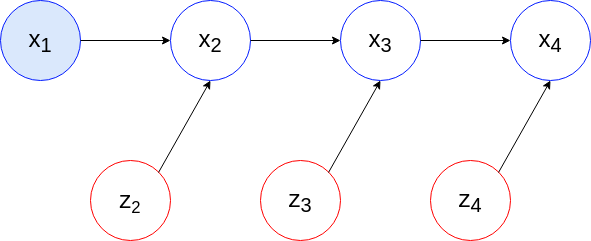
\includegraphics[scale=0.3]{factor_graph.png}
  \caption{Factor Graph of the Problem}
  \label{fig:fac}
\end{figure}

%From the belief computing in (b), the most likely sequence of weather for Days 2 through 4 is \textbf{\{Sunny, Sunny, Rainy\}}. The probability of this sequence is the product of beliefs $ Bel(x_2) \text{ to } Bel(x_4)$, which is \textbf{0.775}.
\end{itemize}

\end{document}

